%
% teil1.tex -- Beispiel-File für das Paper
%
% (c) 2020 Prof Dr Andreas Müller, Hochschule Rapperswil
%
\section{Beschrieb des Zuordnungsproblems
\label{munkres:section:teil1}}
\rhead{Problemstellung}

Das Spezielle an einem Zuordnungsproblem ist, dass es an jedem Ort nur eine Einheit angeboten bzw. nachgefragt wird. Es werden hier nicht Mengen möglichst kostenminimal von einem zum anderen
Ort transportiert, sondern es geht um die kostenminimale Zuordnung von z.B. Personen, oder Bau-Maschinen auf bestimmte Orte, Stellen oder Aufgaben.
Um dieses Problem in einer einfachen, händischen Art und Weise zu lösen wurde der Munkres-Algorithmus, auch die Ungarische Methode genannt, entwickelt. Diese Methode ist ein weiteres Hauptthema dieses Kapitels.

\subsection{Zuordnungsproblem an einem konkreten Beispiel
\label{munkres:subsection:bonorum}}
Man hat den Fall, wo ein Bauunternehmer einen Bauingenieur beauftragt, eine optimale Transportroute für die Umplatzierung seiner Kräne zu eruieren. Das heisst, die Transportstrecke für die Umplatzierung seine Kräne
soll möglichst klein werden. 
Die Frage lautet, wie sind die Kräne umzusetzen, damit deren Transportstrecke minimal wird? Bei der normalen Optimierung dürfen normalerweise beliebige reelle Werte $\mathbb{R}$ angenommen werden. 
Beim Beispiel mit den Kräne gibt es aber ein Problem. Bei der Suche nach der optimalen Lösung darf  nur die Methode der ganzzahligen Optimierung gewählt werden. Materialien kann man aufteilen, jedoch Maschinen nicht. Die Bauarbeiter auf der neuen Baustelle benötigen einen ganzen Kran und nicht nur einen halben Kran. Es muss immer ein ganzer Kran von A nach B oder gar kein Kran verschoben werden. Also 1 oder 0.
Für solche Optimierungsprobleme für reelle Variablen sind verschiedene Verfahren entwickelt worden, die im Allgemeinen auch sehr effizient sind. Das reelle Problem ist also in einer einfachen Art und Weise lösbar. Doch das Problem bleibt, wie in der Illustration oben ersichtlich. Es kann mit ganzzahligen Punkten kein Optimum erzielt werden. Das Ziel ist es an das Optimum so nah wie möglich heranzukommen und dies ist eine vergleichsweise träge und langsame Angelegenheit.

\begin{figure}
\centering
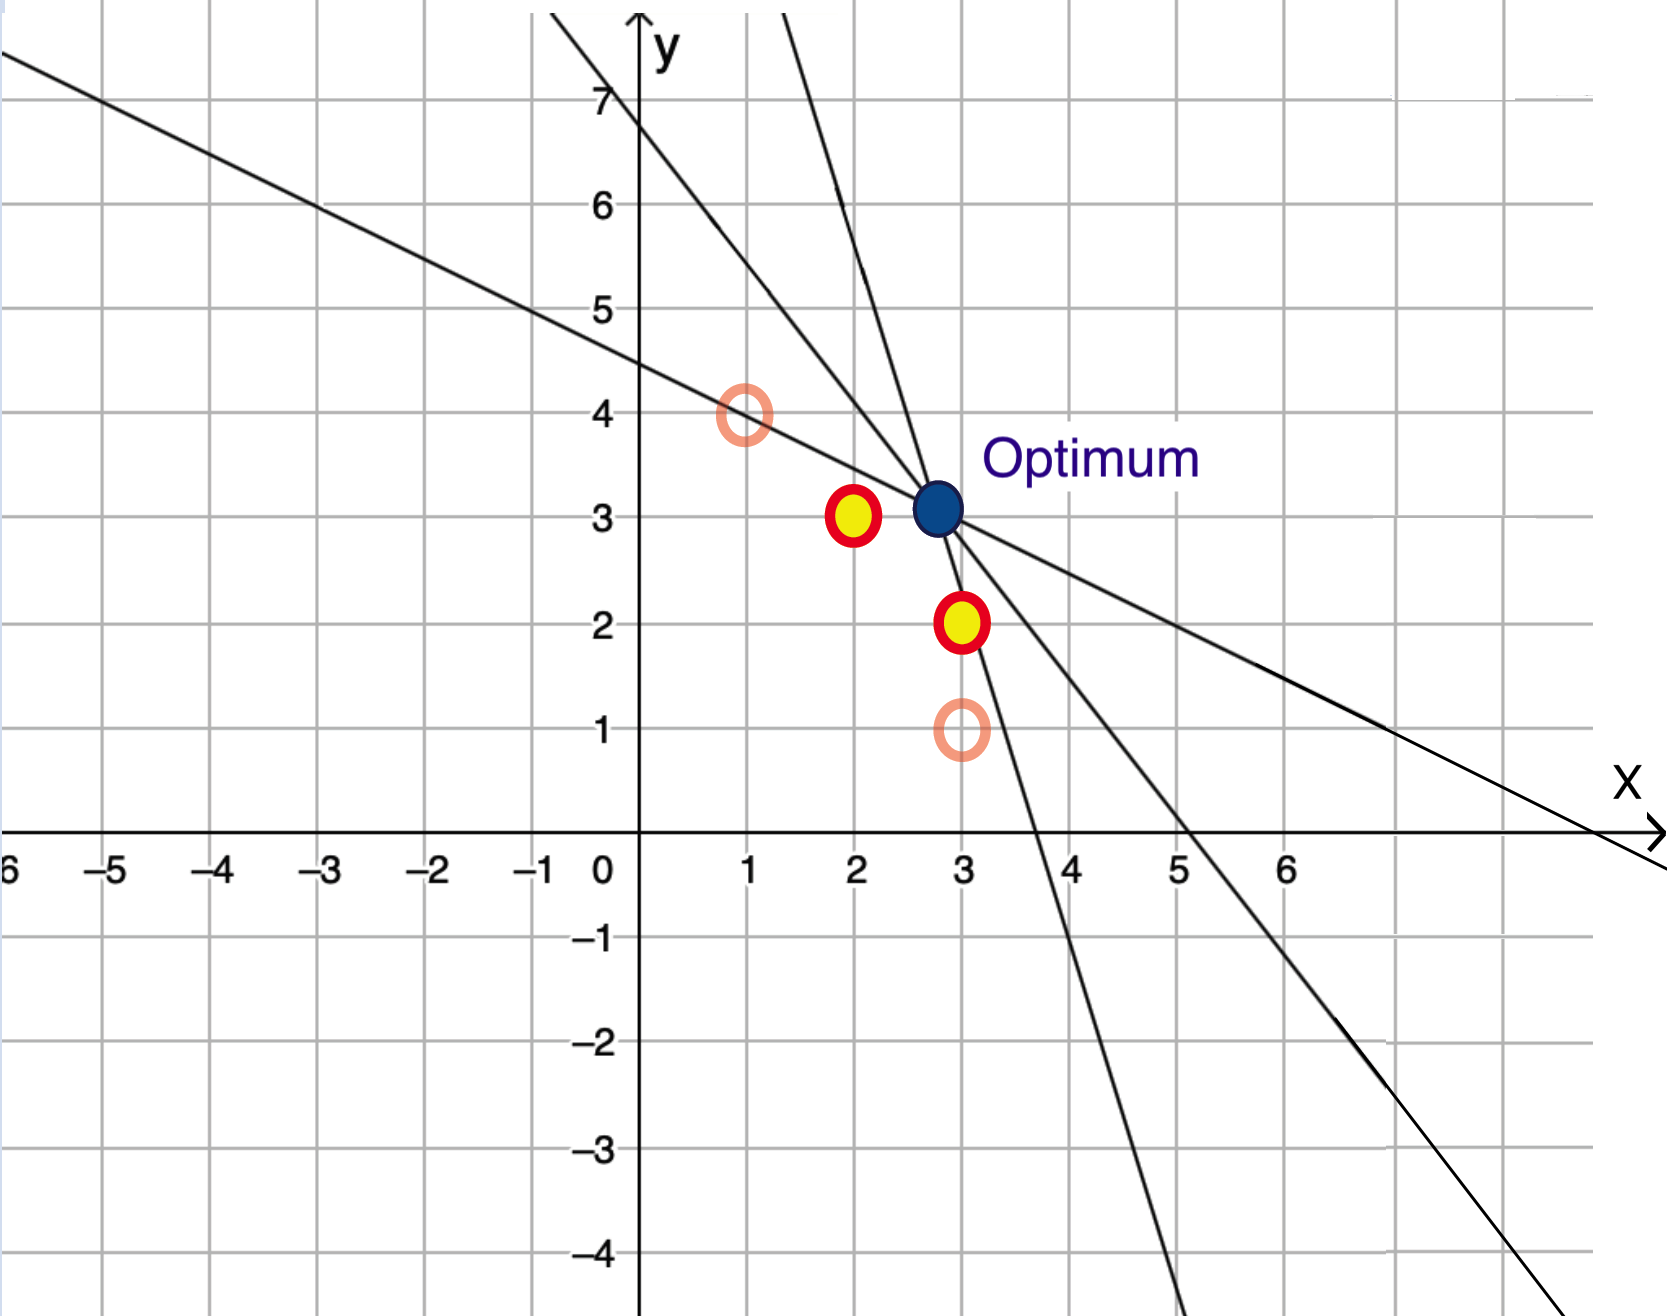
\includegraphics[width=8cm]{papers/munkres/figures/ganzzahlige_punkte}
\caption{Problem der Ganzzahligkeit.}
\label{munkres:Vr2}
\end{figure}


\subsection{Zuordnungsproblem abstrakt
\label{munkres:subsection:bonorum}}

In einem Zuordnungsproblem sind alle Angebots- und Bedarfsmengen gleich 1 
\begin{equation}
a_{i}=b_{j}=1
\end{equation}
Das Ziel ist es die Gesamtkosten zu minimieren. Mit Hilfe einer $n\times n$ Matrix $\mathbb{A}$ $\mathbb{\in}$ $\mathbb{R}^{n,n}$ kann der Faktor Kosten mit in die Rechnung eingebracht werden.
In der Zelle dieser Matrix sind $a_{i,j}$ die Wege dargestellt, die entstehen, wenn man z.B. einem Kran $i$ den Einsatzort $j$ zuordnet.

\begin{figure}
\centering
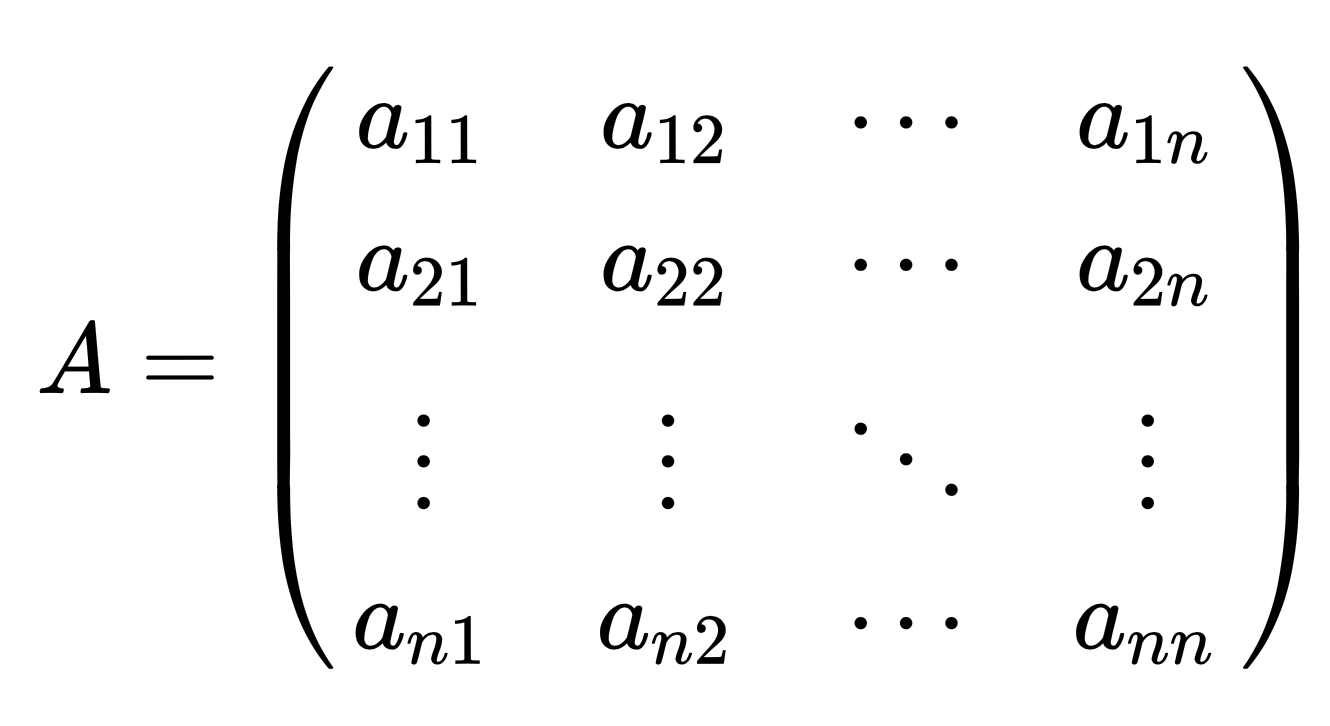
\includegraphics[width=5cm]{papers/munkres/figures/MatrixA.png}
\caption{Darstellung einer Matrix $A$}
\label{munkres:Vr2}
\end{figure}


\subsection{Alternative Darstellungen des Zuordnungsproblems
\label{munkres:subsection:bonorum}}
\begin{equation}
Netzwerk
\end{equation}
\begin{equation}
Matrix
\end{equation}
\begin{equation}
Bitpartiter Graph
\end{equation}
Ein bipartiter Graph ist ein mathematisches Modell für Beziehungen
zwischen den Elementen zweier Mengen.
Es eignet sich sehr gut zur Untersuchung von Zuordnungsproblemen. 
\begin{figure}
\centering
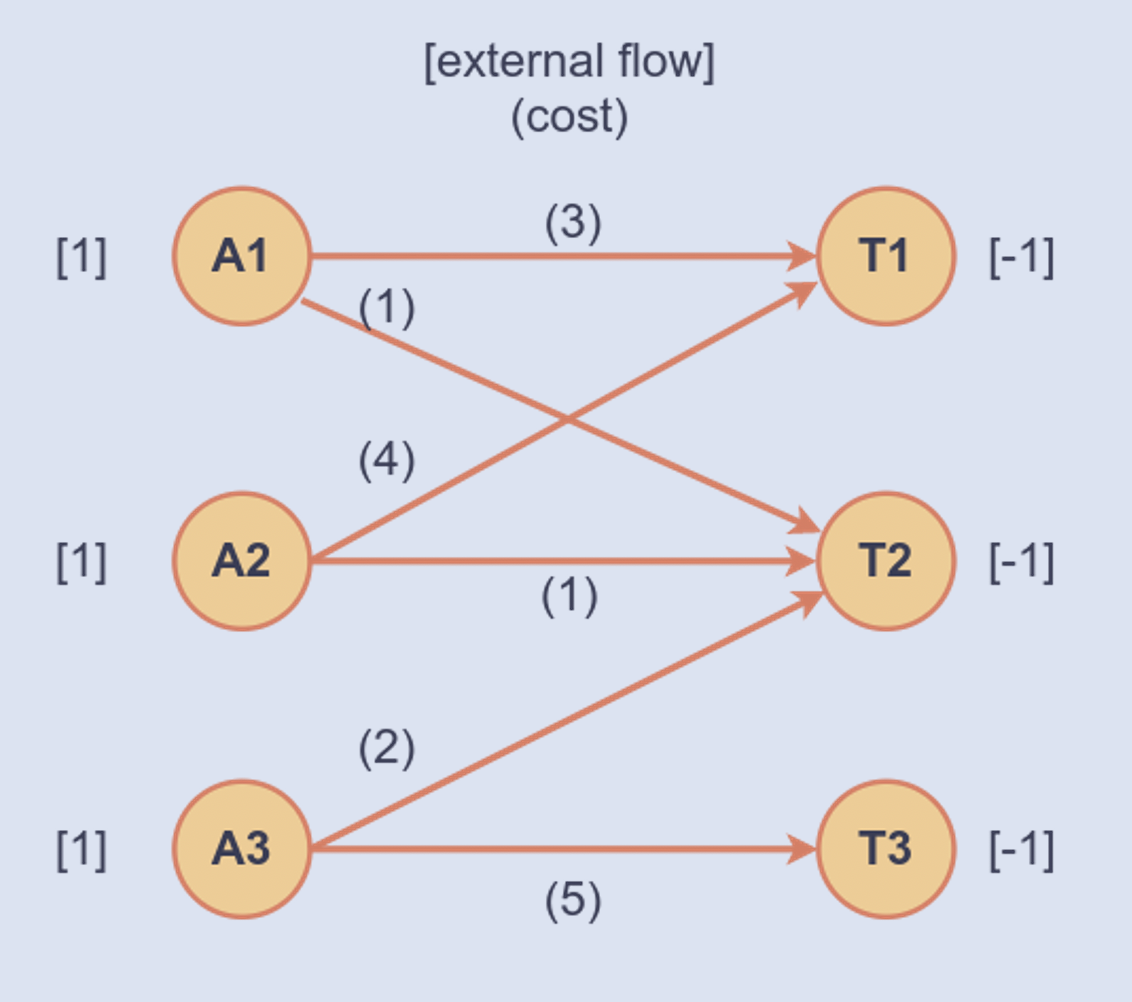
\includegraphics[width=5cm]{papers/munkres/figures/Netzwerkdarstellung}
\caption{Typische Netzwerkdarstellung eines Zuordnungsproblems.}
\label{munkres:Vr2}
\end{figure}

\begin{figure}
\centering
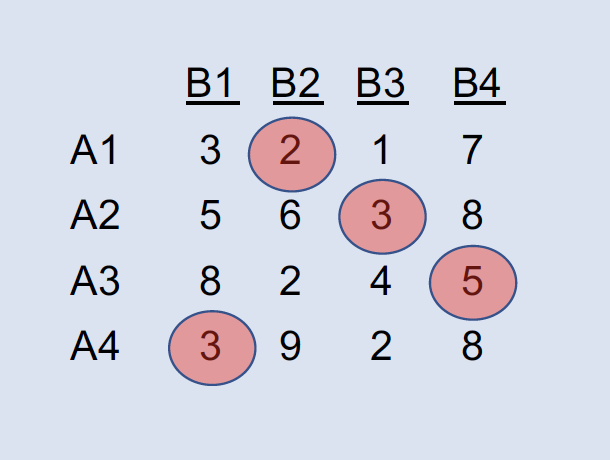
\includegraphics[width=5cm]{papers/munkres/figures/Matrixdarstellung}
\caption{Typische 4x4 Matrixdarstellung eines Zuordnungsproblems.}
\label{munkres:Vr2}
\end{figure}

\begin{figure}
\centering
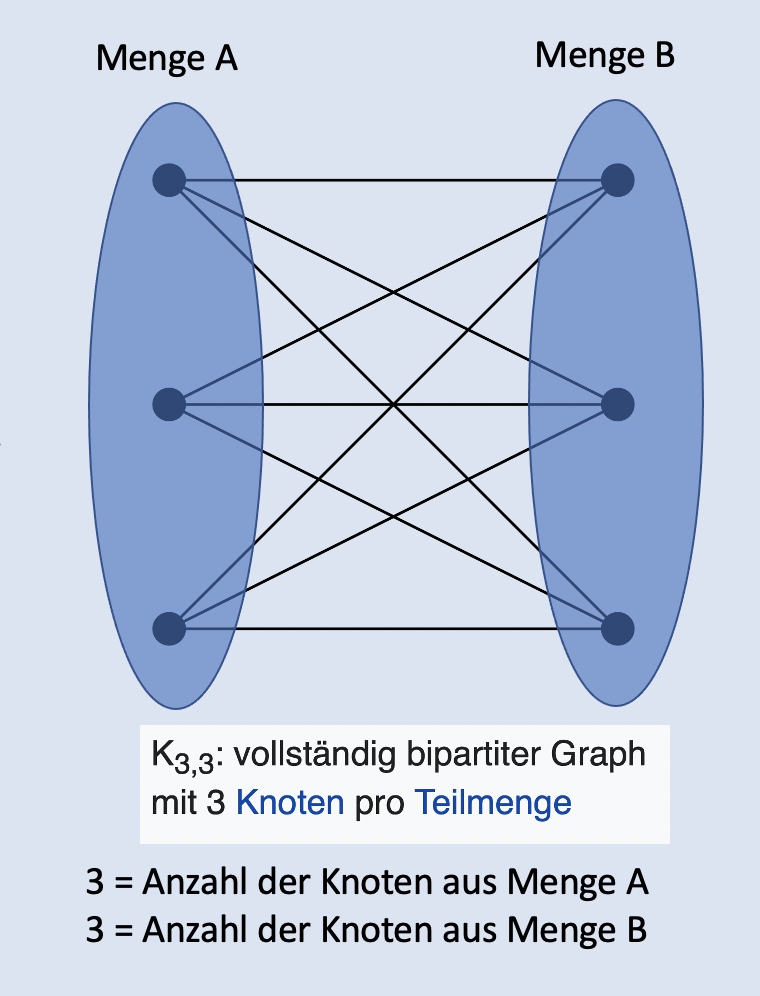
\includegraphics[width=5cm]{papers/munkres/figures/bipartiter_graph}
\caption{$K_{3,3}$ vollständig bipartiter Graph mit 3 Knoten pro Teilmenge.}
\label{munkres:Vr2}
\end{figure}
